%\documentclass[10pt,a4paper]{article}
%\usepackage[latin1]{inputenc}
%\usepackage{amsmath}
%\usepackage{amsfonts}
%\usepackage{amssymb}
%\usepackage{graphicx}

% igs2ejournalguide.tex
% v4.00 3-sept-2015

\NeedsTeXFormat{LaTeX2e}

% check that the math fits the two-column format:
% \documentclass[twocolumn]{igs}

% but use this version when submitting your article:
\documentclass[review,oneside]{igs}

% other options are available
%   authors printing on US letter size are advised 
%   to use the slightly shorter [letterpaper] option
% SINGLE COLUMN
%   \documentclass{igs}              
% SINGLE COLUMN, FEWER LINES/PAGE
%   \documentclass[letterpaper]{igs} 
% DOUBLE COLUMN, FEWER LINES/PAGE
%   \documentclass[twocolumn,letterpaper]{igs} 

\usepackage{igsnatbib}
\usepackage{appendix}

% check if we are compiling under latex or pdflatex
\ifx\pdftexversion\undefined
\usepackage[dvips]{graphicx}
\else
\usepackage[pdftex]{graphicx}
\usepackage{epstopdf}
\epstopdfsetup{suffix=}
\fi

% the default is for unnumbered section heads
% if you really must have numbered sections, remove
% the % from the beginning of the following command
% and insert the level of sections you wish to be
% numbered (up to 4):

% \setcounter{secnumdepth}{2}

\begin{document}
\title{Diagnosising the sensitivity of grounding line flux to changes in sub-ice shelf melting}

\author[Zhang and others]{Tong Zhang, Stephen Price, Matthew Hoffman, Xylar Asay-Davis}
\affiliation{%
  Fluid Dynamics and Solid Mechanics Group, Los Alamos National Laboratory, New Mexico, United States, 87545\\
  Correspondence: Tong Zhang 
  $<$tzhang@lanl.gov$>$}
 
\abstract{Motivated by previous work using ice flow models to quantify ice shelf buttressing and its impacts on the flux of ice across the grounding line \citep[e.g.,][]{furst2016,reese2018}, we seek a better physical understanding for how ice dynamics link small ice thickness perturbations, via changes in sub-ice shelf melting, to changes in ice shelf buttressing and ice flux across the grounding line. More specifically, we seek to define one or more ice shelf buttressing ``metrics'' that are readily calculated from standard ice sheet model outputs and are simultaneously informative for diagnosing the sensitivity of grounding line flux to ice thickness at specific locations on an ice shelf. By studying the ice dynamics for both idealized (MISMIP+) and realistic (Larsen C) ice shelves, we find that the first principle stress at perturbation locations is the best overall metric for linking local changes in ice shelf dynamics with changes in the integrated grounding line flux. Unfortunately, this metric only shows a robust relationship with the integrated grounding line flux for regions near the center of an ice shelf; for points too near the grounding line or too near the calving front, no clear relationship exists between any of the readily calculable metrics explored here and changes in grounding line flux. This motivates our exploration of an adjoint-based method for defining grounding line flux sensitivity to local changes in ice shelf geometry. Using the same idealized and realistic test cases, we demonstrate that this method is equivalent to the sensitivity analysis of \citep{reese2018} but requires only a single model adjoint solve. Thus we suggest that the adjoint-based method can provide a model run-time means of analyzing grounding line flux sensitivity to changes in sub-ice shelf melting.}

\maketitle


\section{Introduction}

Marine ice sheets like West Antarctica (and to a lesser extent, portions of East Antarctica) are grounded below sea level and their bedrock would remain so even after full isostatic rebound [REFS]. This and the fact that ice sheets generally thicken inland lead to a geometric configuration that is unstable; a small increase in flux at the grounding line thins the ice there, leading to floatation, a retreat of the grounding line into deeper water, further increases in flux (due to thicker ice), and further thinning and grounding line retreat. This theoretical ``marine ice sheet instability'' mechanism [Mercer,Schoof1] is supported by idealized [Schoof2,MISMIP+?] and realistic ice sheet modeling [Gudmundson,others?] experiments and some studies [Rignot, Joughin] argue that such an instability is currently under way along outlet glaciers of Antarctica's Amundsen Sea Embayment (ASE). The relevant perturbation for grounding line retreat in the ASE is thought to be intrusions of relatively warm, intermediate depth ocean waters onto the continental shelves [ref to recent review papers in Oceanography? or other recent reviews?], which have reduced the thickness and extent of marginal ice shelves via increased submarine melting [REFS]. These reductions are critical because fringing ice shelves restrict the flux of ice across their grounding lines farther upstream -- the so-called ``buttressing'' affect of ice shelves [gudmundssonOLD,gudmundsson2013,GudmundssonAndDeRydtPaperOnLarsenC?] -- which makes them a critical control on ice flux from Antarctica to the ocean.

%It is therefore a big concern at present if the marine-type West Antarctica Ice Sheet (WAIS) will accelerately retreat and cause a significant sea level rise in the near future \citep{joughin2011}. As ice shelves can supply additional resisting forces (buttressing) to ice flow from upstream and thus decrease the ice flux across grounding line (GL), they are critical for stabilizing marine ice sheets from further retreating \citep{gudmundsson2013}. 

%Warm ocean water is getting more evident of being responsible of increased melt at the base of ice shelves in Antarctica \citep{jenkins2018,rintoul2016}. The basal melting decreases ice thickness and reduce the buttressing ability of ice shelf \citep{gagliardini2010}, and can therefore potentially destabilize marine ice sheets. Satellite altimetry measurements have proved this mechanism that ice shelf thickness decrease links glacier acceleration in Antarctica \citep{pritchard2012}. Recent studies also suggested that the thinning of ice shelfves also contributes to the ice dynamic changes of upstream grounded ice sheets \citep{minchew2018}, indicating the importance of ice shelf-ocean coupling in the whole ice sheet dynamics. 
On ice shelves, gradients in hydrostatic pressure are balanced by the primarily extensional flow of ice towards the calving front \citep{schoof2007}[add a more basic ref, like Paterson, Van der Veen?] and, in theory, a one-dimensional ice shelf provides no buttressing \citep{schoof2007,gudmundsson2013}. \textit{SP: I wonder if this requires a monotonic decrease in ice shelf thickness though?} For realistic, three-dimensional ice shelves however,  buttressing results from three main sources: 1) compressive ice flow 2) lateral shear, and 3) ``hoop'' stress \citep{pegler2012}. \textit{For completeness, we should probably briefly describe how each of these contributes to buttressing rather than assume people already know (?). The first two are easy. I'm not sure about the 3rd.} Due to the complex geometries, kinematics, and dynamics of real ice shelves, an understanding of the specific processes and locations that control ice shelf buttressing is far from straigtforward.



Several recent studies apply whole-Antarctic ice sheet models optimized to present-day observations towards improving our understanding for how Antarctica ice shelves limit flux across the grounding line and, by extension, ice dynamics farther inland. \cite{furst2016} ... \textit{add a few more details on their methods here?} ... to identify regions of the ice shelves that are dynamically ``passive'', such that increased submarine melting, or even complete removal of ice in these areas should not significantly alter local or regional ice dynamics or the flux of ice upstream. \cite{reese2018} used perturbation experiments to link small, localized decreases in ice shelf thickness to changes in integrated grounding line flux (GLF), thereby providing a map of GLF sensitivity to local increases in submarine melt rates. 
%SP: After writing this sentence, it occurs to me that something else that we could follow up on at some point is if / how broader patterns of ice thickness change might complicate the interpretation of these simple perturbation experiments. E.g., you can imagine that 1) multiple perturbations in diff. areas of the ice shelf might conflict with one another and have a more complex impact on g.l. flux (e.g., simultaneous perturbations in multiple areas that show both g.l. flux increases and decreases w/ ice thickness perturbations), 2) similar scale perturbations but applied over wider areas (e.g., over an area that is representative of the actual length scale of submarine melt patterns). Maybe this would be implicit in any 2nd or later study where we perturbed ice shelves based on the sensitivity maps we derive from the adjoint method.

Motivated by these (and other? which?) studies, we build on and extend the methods and analysis of Furst et al. and Reese et al. in order to make progress towards answering the following questions: 
(1) How do local and regional changes in ice shelf geometry affect affect distal changes in GLF? (2) Can local or regional ice shelf dynamics explain GLF sensitivity to local or regional changes in ice shelf thickness? (3) Can we derive and define new tools and analyses for understanding how observed or modeled spatial patterns in submarine melting influence GLF and, by extension, project how changes in submarine melt pattern and magnitude will impact GLF in the future?     

% OLDER: In this study we aim to further improve the understanding of how changes in submarine melting impact grounding line flux, and by inference, marine ice sheet stability. Using both idealized  (MISMIP+; Fig \ref{mismip_larsenc}a) and realistic (Larsen C; Fig \ref{mismip_larsenc}b) ice shelf geometries, we conduct model perturbation experiments similar to those of \cite{reese2018}. Our goal is to better understand the ice dynamical processes linking a local perturbation in ice shelf thickness (via submarine melt changes) to a change in grounding line flux. \textit{SP: I'm not sure if we actually do contribute much to this understanding though, so we might need to refocus this depending on what we actually include in the final version of the paper.} In addition, we explore diagnostics for quantifying grounding-line-flux sensitivity as a function of changes in submarine melt with an eye towards defining quantitative sensitivity ``metrics'' that are readily calculated from standard ice sheet model outputs. 

Below, we first provide a brief description of the ice sheet model used in our study. We follow with a description of the model experiments and a discussion of the experimental results and their interpretation. We then demonstrate and discuss the pros and cons of a number of possible metrics for quantifying GLF sensitivity to changes in submarine melt. Based on limitations in all metrics explored here, we conclude by proposing and demonstrating an adjoint-based calculation that provides a sensitivity map analogous to that from the \cite{reese2018} perturbation experiments but at the cost of a single model adjoint solve.

\begin{figure}
\centering
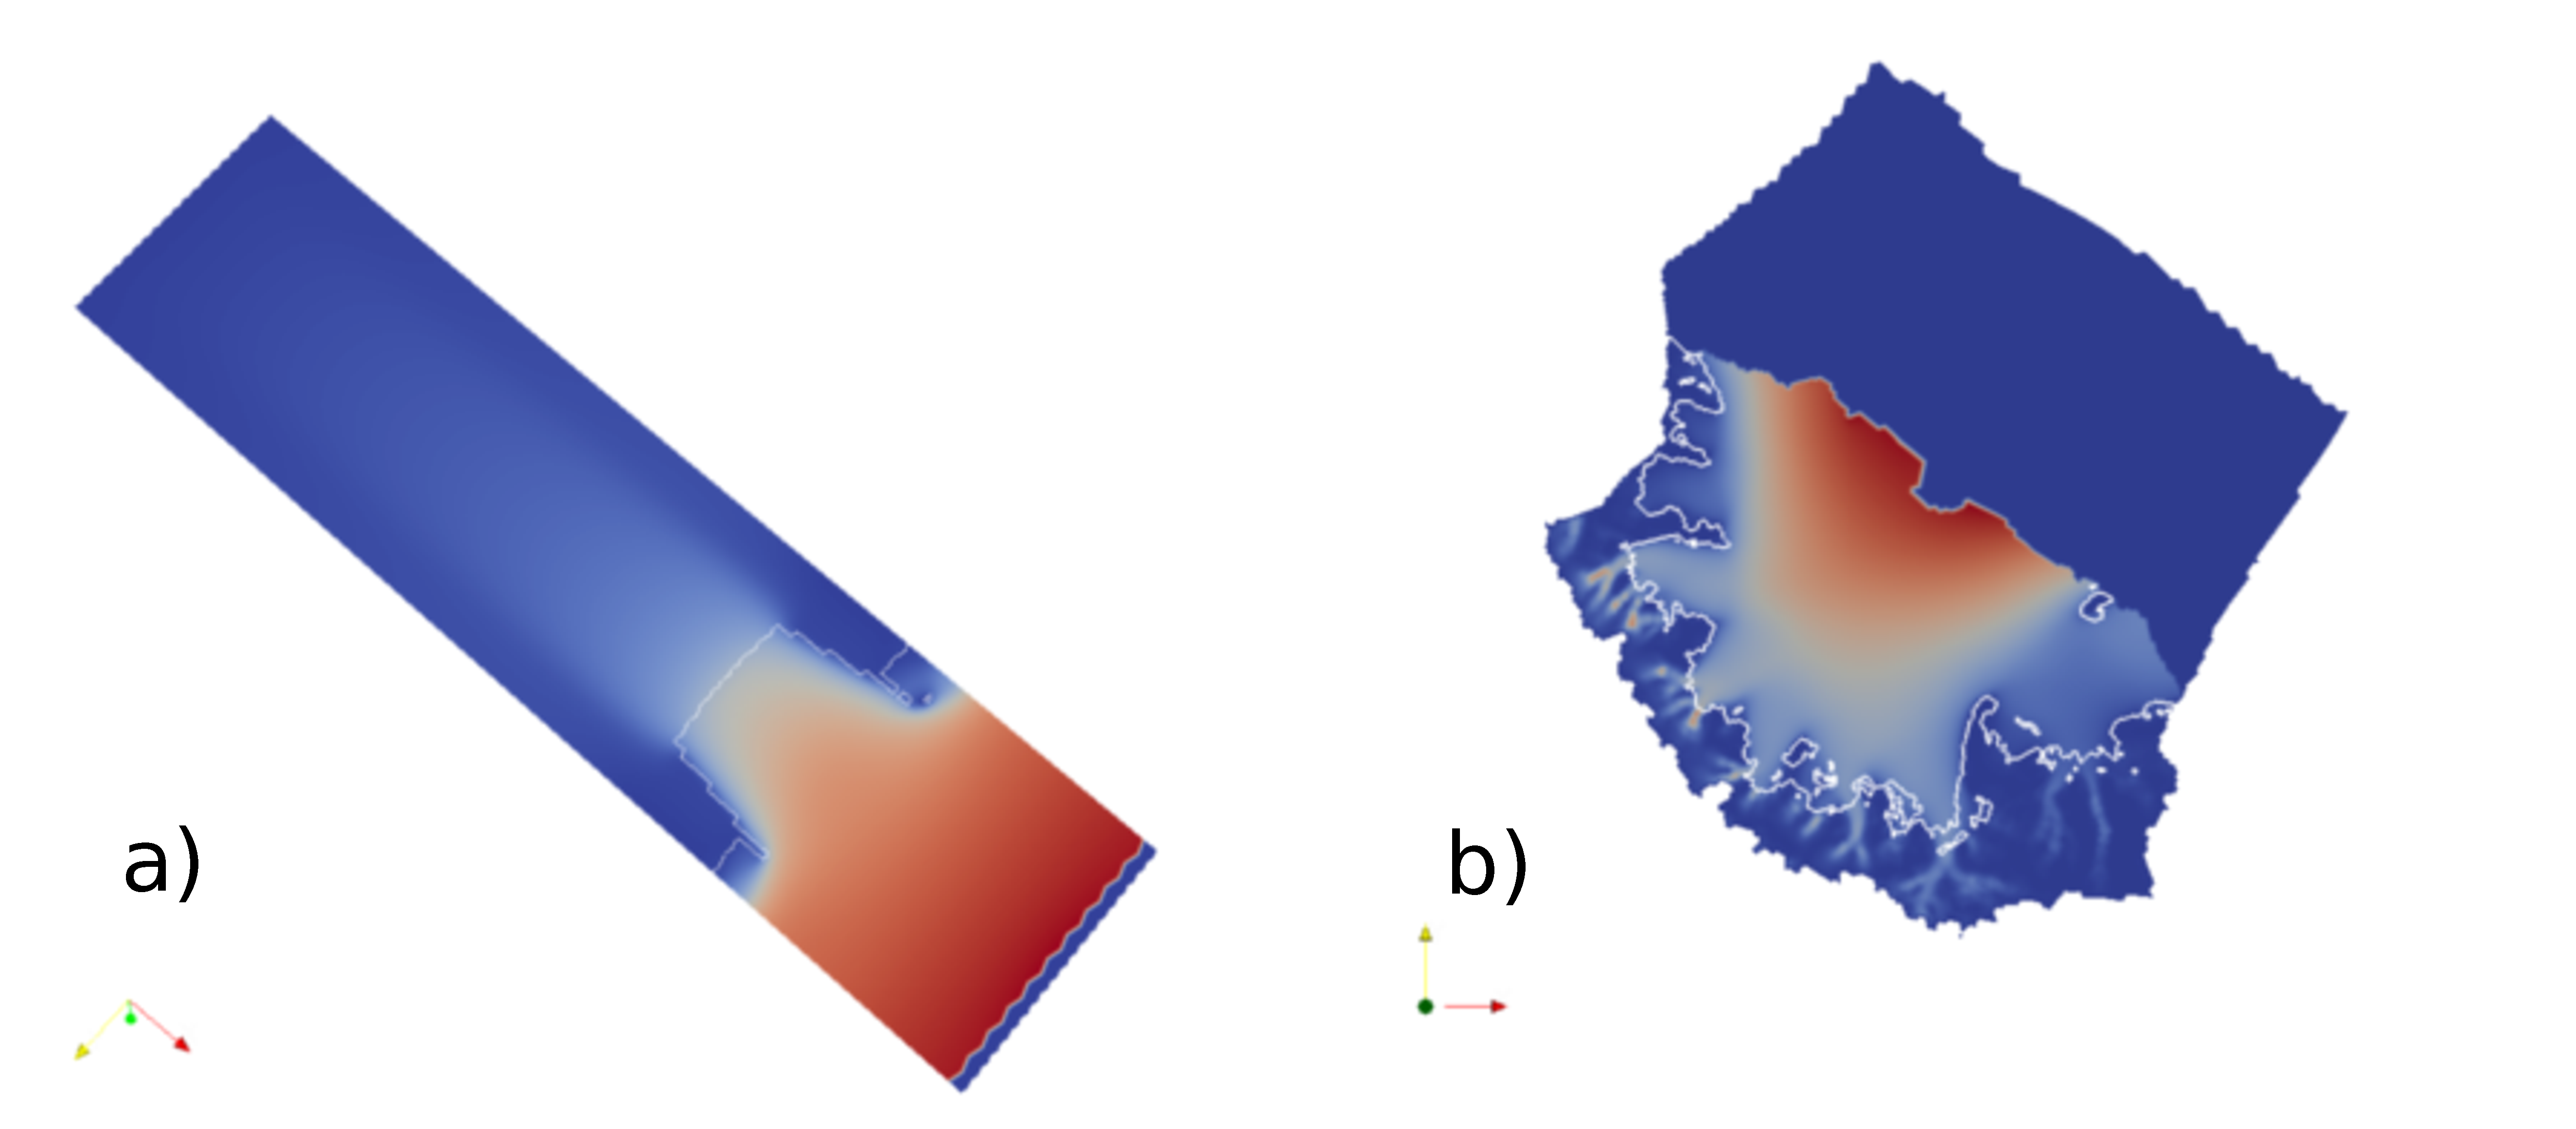
\includegraphics[width=1\linewidth]{figs/mismip_larsenc.pdf}
\caption{Plan view of surface ice speeds for MISMIP+ (a) and Larsen C ice shelf (b). The white curves show the grounding lines.}
\label{mismip_larsenc}
\end{figure}

\section{Model description}
\textit{SP: I built out this section a bit more. We can reduce later on if needed but it seemed a bit too thin. Note that this is mostly copied and lightly edited from the MALI paper, so we'll have to look over carefully and make sure it doesn't end up looking self-plagiarized.}
We use the MPAS-Albany Land Ice model (MALI; \cite{hoffman2018}), which solves the three-dimensional, first-order approximation to the Stokes momentum balance for ice flow\footnote{See \citet{schoof2013} for for a full description of the Stokes momentum balance for ice flow and its lower-order approximations.}. Using the notation  of \cite{perego2012} and \citet{tezaur2015a} this can be expressed as, 
\begin{equation} \label{eq:foStokes}
\left\{
\begin{array}{rcl} -\nabla \cdot (2 \mu_e \dot{\boldsymbol{\epsilon}}_1) + \rho_{i} g
\frac{\partial s}{\partial x}&=&0, \\
-\nabla \cdot (2 \mu_e \dot{\boldsymbol{\epsilon}}_2) +\rho_{i} g
\frac{\partial s}{\partial y} &=& 0, \\
\end{array}\right.
\end{equation}
where $x$ and $y$ are the horizontal coordinate vectors in a Cartesian reference frame, $s(x,y)$ is the ice surface elevation, $\rho_{i}$ represents the ice density, $g$ the acceleration due to gravity, and $\dot{\boldsymbol{\epsilon}}_{1,2}$ are the two dimensional strain rate vectors given by
\begin{equation}
\dot{\boldsymbol{\epsilon}}_1 = \left(\begin{array}{ccc}
2\dot{\epsilon}_{xx} + \dot{\epsilon}_{yy}, &\dot{\epsilon}_{xy},&
\dot{\epsilon}_{xz}\end{array}\right)^T,
\end{equation}
and
\begin{equation}
\dot{\boldsymbol{\epsilon}}_2 = \left(
\begin{array}{ccc}\dot{\epsilon}_{xy}, &
\dot{\epsilon}_{xx} + 2\dot{\epsilon}_{yy}, &\dot{\epsilon}_{yz}
\end{array}\right)^T.
\end{equation}
The ``effective'' ice viscosity, $ \mu_e$ in Equation \ref{eq:foStokes}, is given by 
\begin{equation}
\label{eq:effvisc}
    \mu_{e}~=~\gamma A^{-\frac{1}{n}}\dot{\epsilon}_{e}^{\frac{1-n}{n}},
\end{equation}
where $\gamma$ is an ice stiffness factor, $A$ is a temperature-dependent rate factor, $n=3$ is the power-law exponent, and the effective strain rate, $\dot{\epsilon}_{e}$, is defined as
\begin{equation} \label{eq:effstrain}
\dot{\epsilon}_e \equiv \left( \dot{\epsilon}_{xx}^2 +
\dot{\epsilon}_{yy}^2 + \dot{\epsilon}_{xx} \dot{\epsilon}_{yy} +
\dot{\epsilon}_{xy}^2 + \dot{\epsilon}_{xz}^2 +
\dot{\epsilon}_{yz}^2 \right)^\frac{1}{2}.
\end{equation}
Gradients in the horizontal velocity components, $u$ and $v$, contribute to the individual strain rate terms in Equation \ref{eq:effstrain} and are given by
\begin{equation} \label{eq:epsilonij}
\dot{\epsilon}_{xx} = \frac{\partial u}{\partial x}, \hspace{0.5cm} 
\dot{\epsilon}_{yy} = \frac{\partial v}{\partial y}, \hspace{0.5cm}
\dot{\epsilon}_{xy} = \frac{1}{2}\left(\frac{\partial u}{\partial y} + \frac{\partial v}{\partial x} \right), \hspace{0.5cm}
\dot{\epsilon}_{xz} = \frac{1}{2} \frac{\partial u}{\partial z}, \textrm{ and } \hspace{0.15cm} 
\dot{\epsilon}_{yz} = \frac{1}{2} \frac{\partial v}{\partial z}.
\end{equation}

A stress free upper surface is enforced through 
\begin{equation} \label{eq:stressFreeBC}
\dot{\boldsymbol{\epsilon}}_1 \cdot \mathbf{n} = \dot{\boldsymbol{\epsilon}}_2 \cdot \mathbf{n} = 0, 
\end{equation}
where $\mathbf{n}$ is the outward pointing normal vector at the ice sheet upper surface, $z=s(x,y)$.
The lower surface is allowed to slide according to the continuity of basal tractions,
\begin{equation} \label{eq:basalbc}
\begin{array}{ll}
2\mu_e \dot{\boldsymbol{\epsilon}}_1 \cdot \mathbf{n} + \beta u = 0, \hspace{0.2cm} 2 \mu \dot{\boldsymbol{\epsilon}}_2 \cdot \mathbf{n} + \beta v = 0, \\
\end{array}
\end{equation}
where $\beta$ is a spatially variable, linear-friction coefficient. On lateral boundaries in contact with the ocean, the portion of the boundary above sea level is stress free while the portion below sea level feels the ocean hydrostatic pressure according to
\begin{equation}\label{eq:oceanbc}
\begin{array}{ll}
2 \mu_e \left(\dot{\boldsymbol{\epsilon}}_1 \cdot \mathbf{n},\, \dot{\boldsymbol{\epsilon}}_2 \cdot \mathbf{n},\, 0\right)^T -\rho_i g (s-z)\mathbf{n} = \rho_o g \max(z,0) \mathbf{n},
\end{array}
\end{equation}
where $\rho_o$ represents the density of ocean water and $\mathbf{n}$ the outward pointing normal vector to the lateral boundary (i.e., parallel to the $(x,y)$ plane). 

A more complete description of the full MALI model, including the implementations for mass and energy conservation, can be found in \cite{hoffman2018}. Additional details about the Albany momentum balance solver can be found in \cite{tezaur2015a,tezaur2015b}. 

Here, we apply MALI to experiments on both idealized and realistic marine-ice sheet geometries. For our idealized domain and model state, we start from the equilibrium initial conditions for the MISMIP+ experiments, as described in \cite{asay2016} and Cornford and others (MISMIP+ papers). The model mesh is spatially uniform at 2 km resolution. For our realistic domain, we use Antarctica's Larsen C ice shelf and its upstream catchement area. The model state is based on the optimization of the ice stiffness ($\gamma$ in Equation \ref{eq:effvisc}) and basal friction ($\beta$ in Equation \ref{eq:basalbc}) coefficients to match present-day velocities \citep{rignot2014} using adjoint-based methods discussed in \cite{hoffman2018} and \cite{perego2014}. The domain geometry is based on BEDMAP2 \citep{fretwell2013} and ice temperatures, which are held fixed for this study, are based on \cite{liefferinge2013}. Mesh resolution coarsens to 20 km in the ice sheet interior and is no greater than 6 km within the ice shelf \textit{This seems coarse to me ... don't we go to finer resolution, e.g. 2 km, near the g.l.?}. Following optimization to present-day velocities, the model is relaxed using a 100 year forward run and it is this initial condition from which the experiments discussed below are conducted. Both the MISMIP+ and Larsen C experiments use 10 vertical layers that are finest near the bed and coarsen towards the surface (4\% and 23\% of the total thickness, respectively). The grounding line position is determined from hydrostatic equilibrium and a sub-element parameterization analogous to method SEP3 from \cite{seroussi2014} is used to define basal friction coefficient values at the grounding line. 

% For the idealized MISMIP+ experiments, we use its  steady-state geometry following the same model configurations as in \cite{asay2016}. The mesh is spatially uniform (2 km). Both MISMIP+ and Larsen C experiments use 10 vertical layers that are finest near the bed (4\% of total thickness) and coarsen towards the surface (23\% of total thickness).

\section{Perturbation experiments}

To explore the sensitivity of changes in GLF to small changes in ice shelf thickness, we conduct a number of perturbation experiments analagous to those of \citet{reese2018}. Using diagnostic model solutions, we first study the instantaneous response of GLF for the idealized geometry and initial state provided by the MISMIP+ experiment \citep{asay2016}. We then conduct a similar study but using a realistic configuration and initial state for Antarctica's Larsen C ice shelf. %{\bf{possibly add more real ice shelves?}})

Our experiments are conducted in a manner similar to those of \cite{reese2018}. We perturb the coupled ice sheet-shelf system by decreasing the ice thickness uniformly by 1 m over square grid ``boxes'' covering the base of the ice shelves, after which we examine the instantaneous impact on kinematics and dynamics (discussed further below). For MISMIP+, the uniform, 2 km mesh implies that grid cell centers naturally align with these boxes. For the Larsen C ice shelf, horizontal mesh resolution is spatially variable and we assign each grid cell to fall within one and only one box based on its location. For MISMIP+, we use both 2$\times$2 km and 10$\times$10 km square boxes in order to additionally investigate the impacts of spatially averaging perturbations over larger areas. For Larsen C, we only use 20$\times$20 km square boxes (i.e., as in \citet{reese2018}). Lastly, for the MISMIP+ 2 km experiments we note that, in order to save on computing costs, we only perturb the region of the ice shelf for which $x<530$ km (the area over which the ice shelf is likely lateraly buttressed) and $y>40$ km (one half of the ice shelf due to the symmetry about the centerline).

Similar to \cite{reese2018}, we define a GLF response number
\begin{equation}
N_r = \left(\frac{R}{P}\right)^k,
\end{equation}
where $R$ is the ice flux change integrated along the entire grounding line, $P$ is the mass associated with a single grid box perturbation (e.g.,2 km$\times$2 km $\times$0.001 km for the MISMIP+ perturbation experiments) and $k$ is a power-law index that allows for the possiblity of a nonlinear relationship between ice shelf buttressing and the change in GLF (see also \cite{schoof2007}). Here, we use $k=1/n$ ($n=3$).

Despite many different factors (ice flow directions, horizontal gradients of ice shelf geometry, stress fields, strain-rate fields, perturbation locations, etc) existing, we here mainly present the results of the stress fields and the distances between perturbations and GL, as they appears to correlate more closely to the sensitivity of GL flux change to ice shelf perturbations. Similar to  \cite{furst2016} (Eqn \ref{butN}), we calculate buttressing numbers ($N_b$) for 8 different stress components, i.e., normal stresses along ($\sigma_f$) and across flow ($\sigma_{af}$), first ($\sigma_{p1}$) and second ($\sigma_{p2}$) principle stresses, normal stress along the $x$ ($\sigma_{x}$) and $y$ direction ($\sigma_{y}$), shear stress ($\sigma_s$) and hoop stress ($\sigma_h$), and get their corresponding GL flux response numbers,
\begin{equation}
N_b=1-\frac{\sigma_{obj}}{N_0},
\label{butN}
\end{equation}
where $N_0$ is the vertically integrated ocean pressure ($N_0=0.5\left(1-{\rho_i}/{\rho_w}\right)gH$). $\rho_i$ (910 kg m$^3$) and $\rho_w$ (1028 kg m$^3$) are the density of ice and ocean water, respectively. Table 1 lists these 8 different buttressing number ($\sigma_{obj}$) definitions, where $n_f$, $n_{af}$, $n_x$ and $n_y$ are the unit vector components of the ice flow and coordinate direction, $H$ is the ice thickness, $u$ is the radial flow velocity and $r$ is the radial axis coordinate. Hoop stress arises from regions where ice flow is divergent, and is another source of ice shelf resistence except for compression and lateral shearing of ice flow \citep{pegler2012, wearing2016}.

\begin{table*}
\centering
\caption{Stress components used in the buttressing (Eqn \ref{butN})}
\label{stressDef}
\begin{tabular}{|c|c|c|c|}
\hline
$\sigma_{obj}$ & def. & $\sigma_{obj}$ & def. \\
\hline
$\sigma_f$ & ${\bf{n}}^T_f\cdot{\bf{\sigma}}\cdot{\bf{n}}_f$ & $\sigma_{af}$ & ${\bf{n}}^T_{af}\cdot{\bf{\sigma}}\cdot{\bf{n}}_{af}$ \\ 
\hline 
$\sigma_{x}$ & ${\bf{n}}^T_x\cdot{\bf{\sigma}}\cdot{\bf{n}}_x$ & $\sigma_{y}$ & ${\bf{n}}^T_y\cdot{\bf{\sigma}}\cdot{\bf{n}}_y$ \\ 
\hline
$\sigma_{p1}$ & $\frac{\sigma_{x}+\sigma_{y}}{2}+\sqrt{\left(\frac{\sigma_{x}-\sigma_{y}}{2}\right)^2+\sigma_{xy}^2}$ & $\sigma_{p2}$ & $\frac{\sigma_{x}+\sigma_{y}}{2}-\sqrt{\left(\frac{\sigma_{x}-\sigma_{y}}{2}\right)^2+\sigma_{xy}^2}$ \\ 
\hline 
$\sigma_s$ & ${\bf{n}}^T_f\cdot{\bf{\sigma}}\cdot{\bf{n}}_{af}$ & $\sigma_h$ & $\eta H\frac{\partial}{\partial r}\left(\frac{u}{r}\right)$ \\ 
\hline

\end{tabular}
\end{table*}

\section{Results}
\subsection{MISMIP+}
Before and after the perturbation, the GL velocity change clearly shows a spatial pattern (Fig \ref{stndVarFluxP}a). By calculating the standard deviation of the velocity change along GL for each 2 km perturbation experiment, we can see that the GL velocity change data is more dispersed for perturbation near GL, while for pertuirbations at the central region of the ice shelf, the corresponding GL velocity change is less variant along GL. If we look at Figure \ref{stndVarFluxP}b, the integrated GL flux is more contributed by the GL cells that close to the perturbation spot, i.e., the neighboring GL cells appears to have more flux contribution weight than those far away from the perperturbation location, and the perturbations near the ice shelf center tend to impact more uniformly on the GL dynamics.

\begin{figure}
\centering
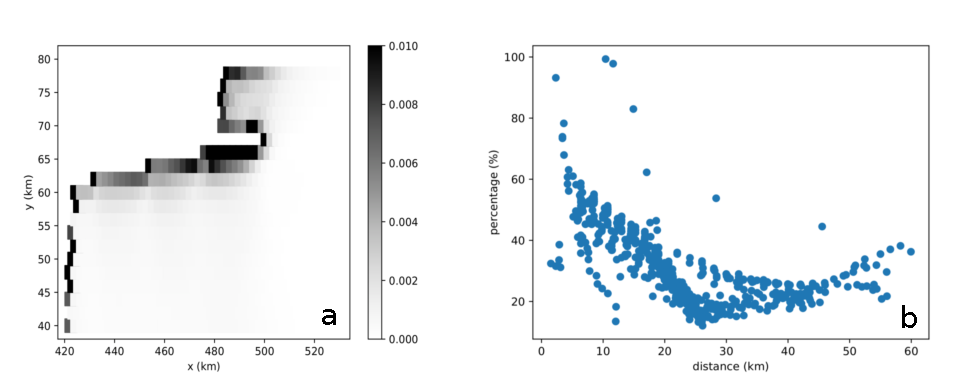
\includegraphics[width=1\linewidth]{figs/stndVarFluxP.pdf}
\caption{(a) The distribution of the standard variance of the ice velocity changes on the grounding line of MISMIP+ for all perturbation experiments (note we only do the perturbation experiments for half space in $y$ of MISMIP+); (b) We find five cells on the grounding line that are the nearset to the perturbation spot. The x-axis is their mean distances to the perturbation box. The y-axis shows their combined flux contribution in the total integrated grounding line flux.}
\label{stndVarFluxP}
\end{figure}

This can be further examined by looking at the relationship between GL flux response number ($N_r$) and the buttressing number ($N_b$) for the first principle stress ($\sigma_{p1}$) at different $dG$ and $dC$ (Fig \ref{diffdCdG}). $dG$ ($dC$) is the minimum distance between perturbation boxes and GL (calving front). When both $dG$ and $dC$ increase, perturbation boxes are farther away from GL and calving front, the velocity changes at GL become less dispersible and their relationship gets less ``noisy'' and tends to show linear trends. The possible explanaions can be found in the following ``Discussions'' section.

\begin{figure}
\centering
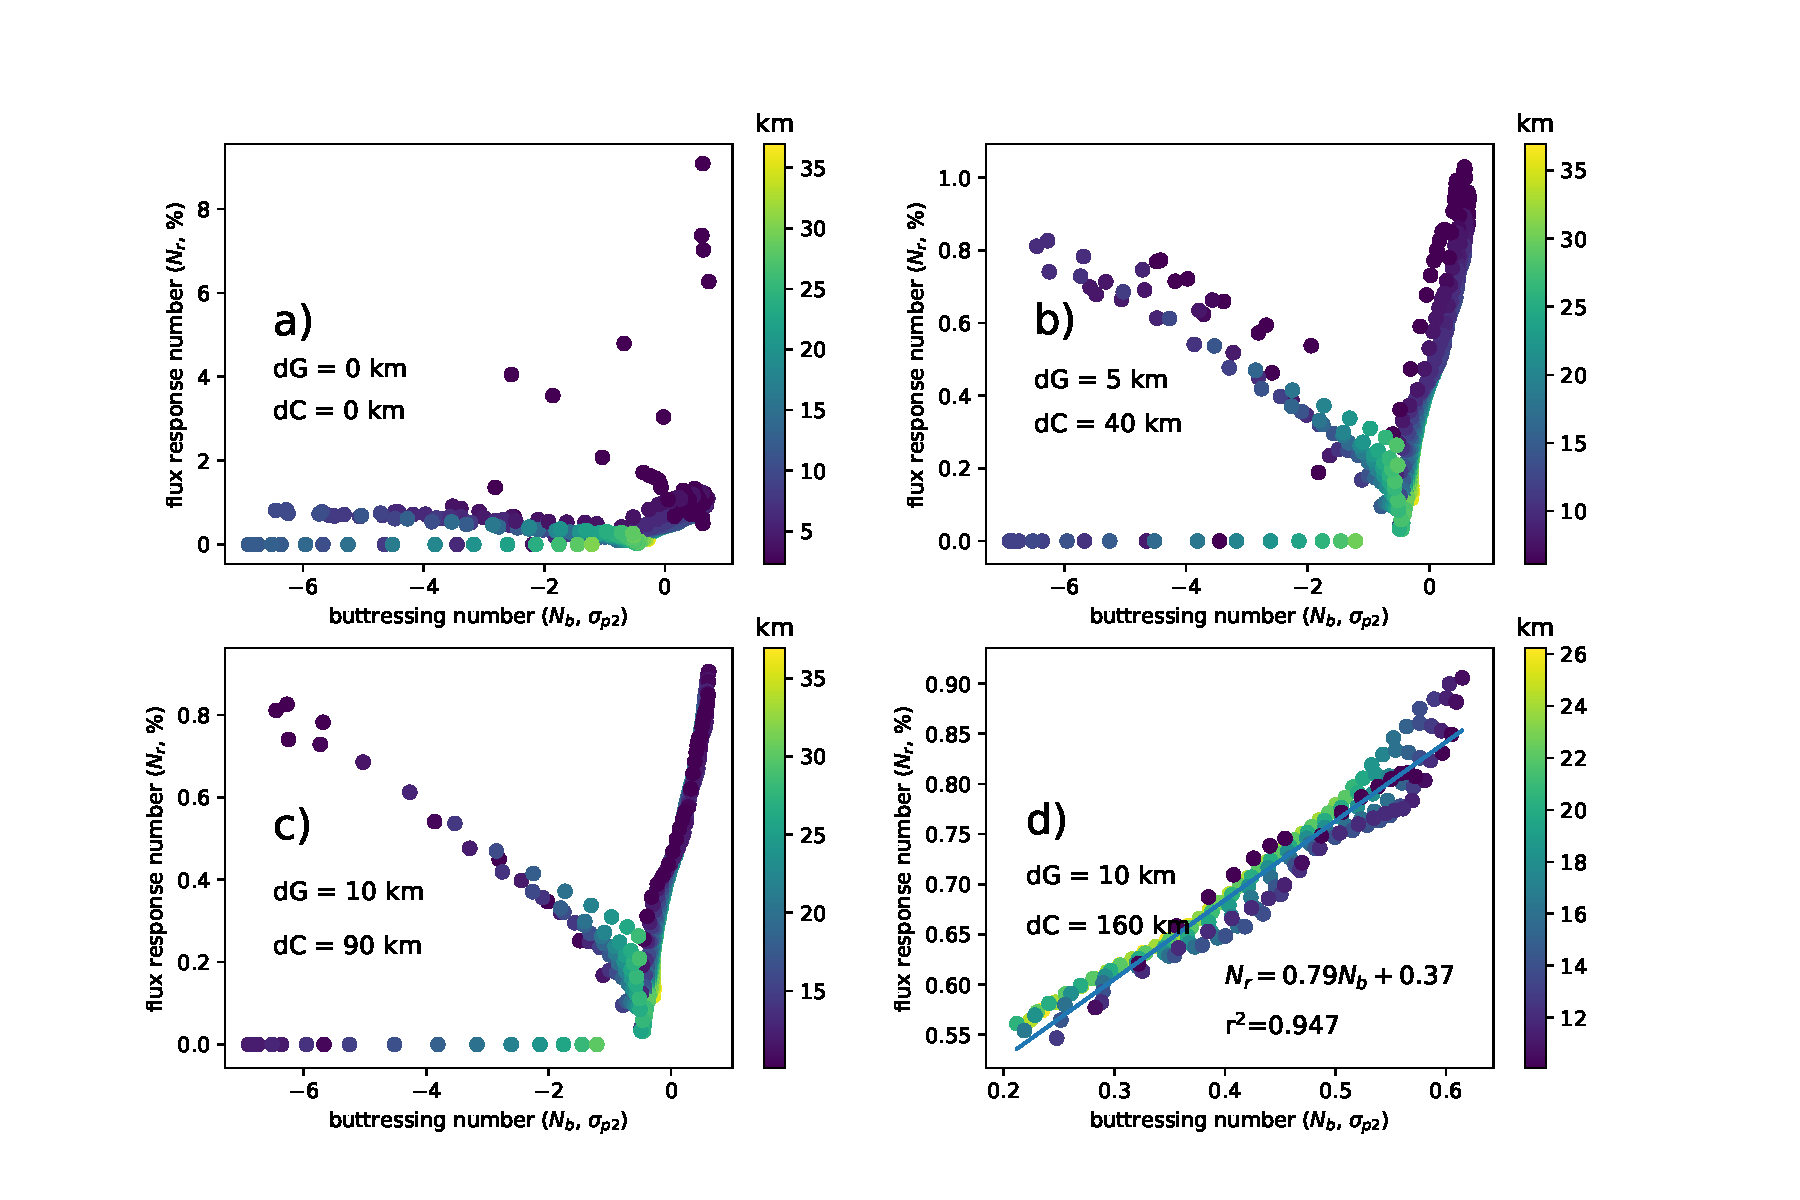
\includegraphics[width=1\linewidth]{figs/diffdCdG.pdf}
\caption{The relationships between the groundling line flux response number ($N_r$) and the buttressing number ($N_b$) at the perturbation spots by different geometric filters of $dG$ and $dC$. Larger $dG$ and $dC$ give perturbation spots that are more centralized in the ice shelf. Smaller $dG$ and $dC$ mean the perturbation locations are either close to the grounding line or the calving front. The color bars show the values of $dG$ for each perturbation spot.}

\label{diffdCdG}
\end{figure}

In fact, $\sigma_{p1}$ appears to be the best metric for predicting such linear relationship, comparing to the other 7 stress components (Fig \ref{diffStressComp}). The $N_b$ for $\sigma_f$, $\sigma_{af}$, $\sigma_x$ and $\sigma_y$ show some weak correlations with GL flux response number $N_b$. The shear stress and hoop stress, however, have no clear evidences of relating to $N_r$. Note that for all plots in Figure \ref{diffStressComp}, we have removed the ``noisy'' perturbation spots using $dG$ and $dC$. It is suprising that $\sigma_{p1}$ shows better performance than $\sigma_{p2}$ and $\sigma_s$, as $\sigma_{p2}$ gives the maximum buttressing number and predicts well the passive ice regions in \cite{furst2016} and the shear stress supply the main large resistence force for divergent ice flow regions (most of the MISMIP+ ice shelf) \citep{wearing2016}.

\begin{figure}
\centering
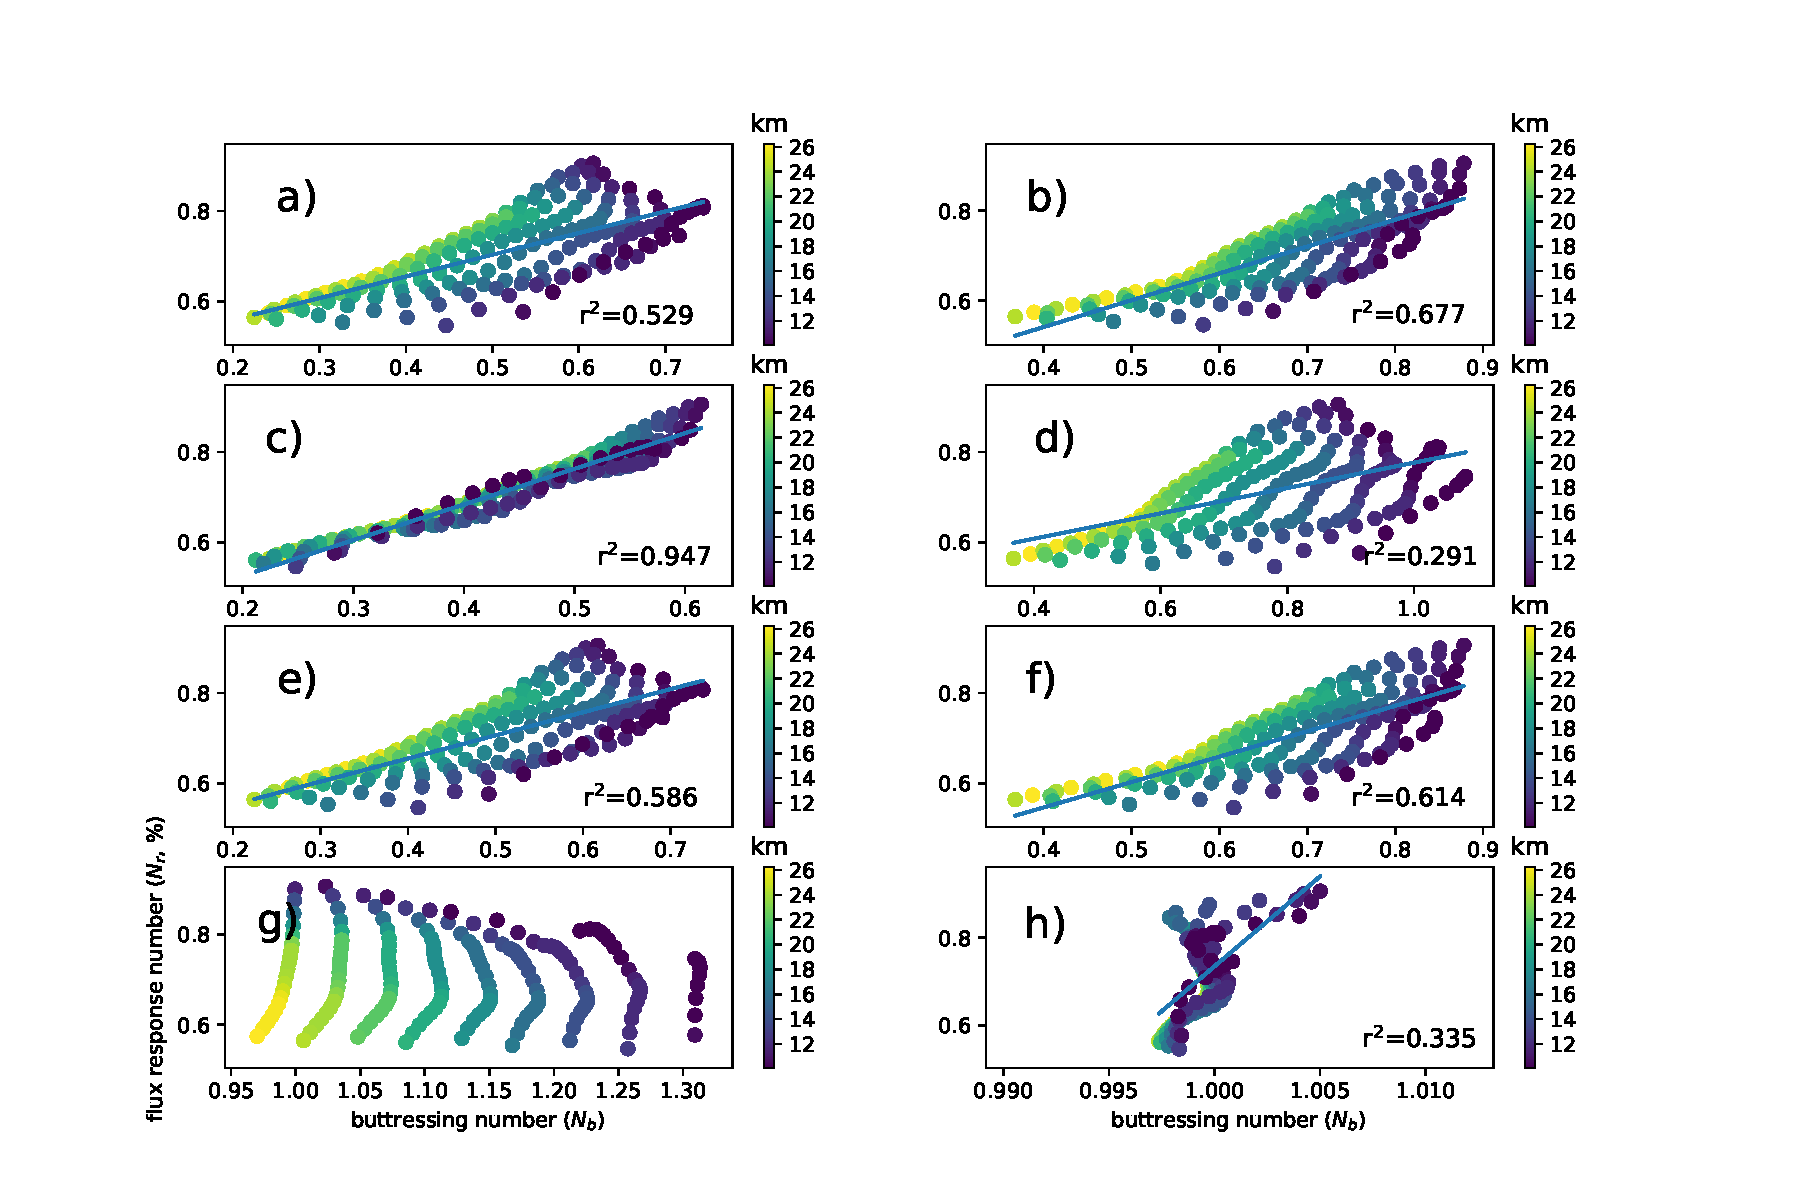
\includegraphics[width=1\linewidth]{figs/diffStressComp.pdf}
\caption{The relationships between grounding line flux response number ($N_r$) and eight different stress components, $\sigma_f$ (a), $\sigma_{af}$ (b), $\sigma_{p1}$ (c), $\sigma_{p2}$ (d), $\sigma_{x}$ (e), $\sigma_{y}$ (f), $\sigma_{s}$ (g) and $\sigma_h$ (h). See Table \ref{stressDef} for the definition of each stress component in the MISMIP+ 2 km $\times$ 2 km box experiments. The color bars show the values of $dG$ for each perturbation spot.}
\label{diffStressComp}
\end{figure}

The buttressing number for $\sigma_{p1}$ also performs well for the 10 km $\times$ 10 km square box perturbation experiments (Fig \ref{diffStressCompAvg}), for which we average the stresses across all cells in each square box. In fact, except the shear stress $\sigma_s$, all correlations are improved compared to the 2 km $\times$ 2 km perturbation experiments. In particular, the hoop stress shows some improved predictability as well. But again, $\sigma_{p2}$ is still not preferable than $\sigma_{p1}$.

\begin{figure}
\centering
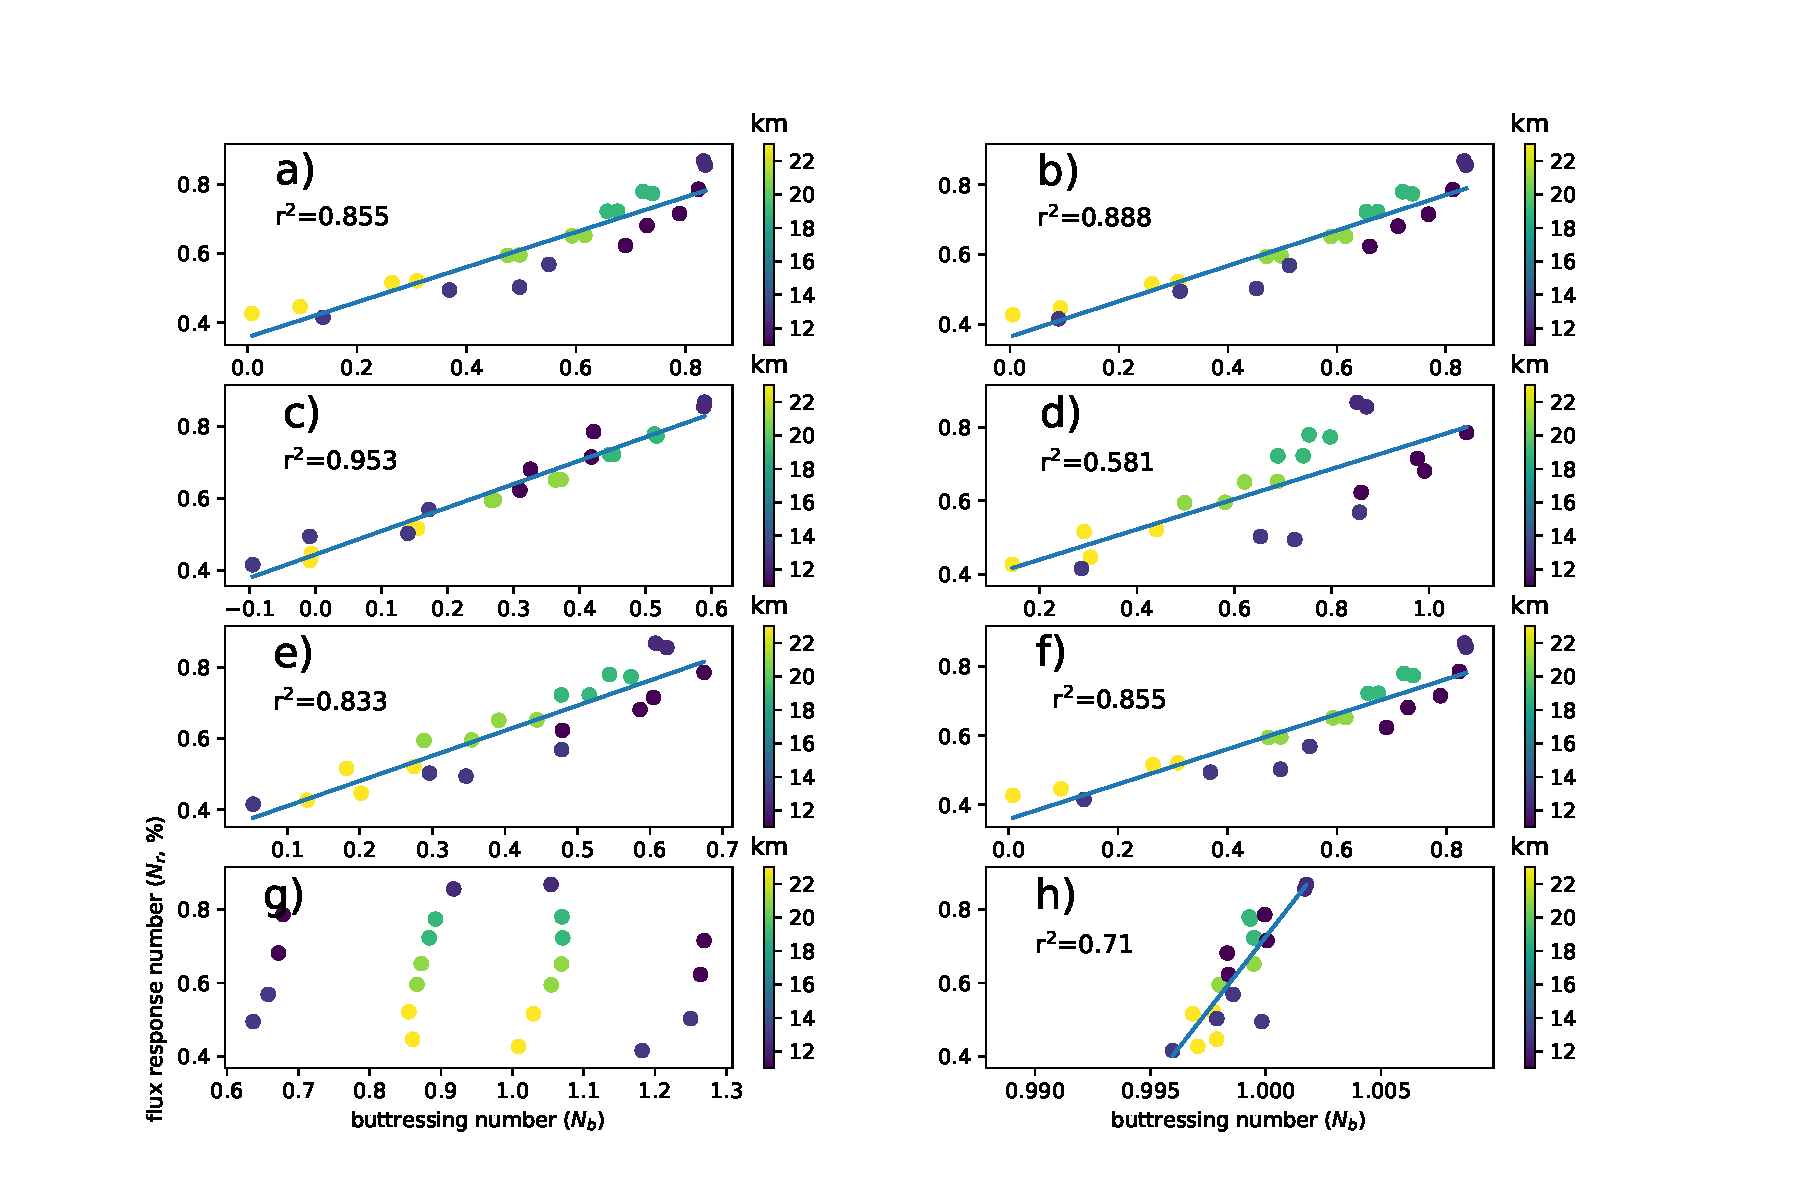
\includegraphics[width=1\linewidth]{figs/diffStressCompAvg.pdf}
\caption{The relationships between grounding line flux response number ($N_r$) and eight different stress components, $\sigma_f$ (a), $\sigma_{af}$ (b), $\sigma_{p1}$ (c), $\sigma_{p2}$ (d), $\sigma_{x}$ (e), $\sigma_{y}$ (f), $\sigma_{s}$ (g) and $\sigma_h$ (h). See Table \ref{stressDef} for the definition of each stress component in the MISMIP+ 10 km $\times$ 10 km box experiments. The color bars show the values of $dG$ for each perturbation spot.}
\label{diffStressCompAvg}
\end{figure}

\subsection{Realistic ice shelves (Larsen C)}

To validate if there are the same $N_b$-$N_r$ patterns as in the MISMIP+ case for realistic ice shelves, we apply the same analysis processes as above for the Larsen C ice shelf. Because the mesh resolution varies from GL to calving front, we apply 20 km $\times$ 20 km square boxes to the perturbation experiments and adjust the box areas by counting actual cell numbers that each box includes. In addition, due to the complex geometry (GL shape and ice rises) of Larsen C ice shelf, we adopt $dG=50$ km and $dC = 50$ km for better removing those near-GL noises. 

From Figure \ref{diffStressCompAvgL}, we can also see good linear $N_b$-$N_r$ relations for most of the stress components, especially for $\sigma_{p1}$, similar to the MISMIP+ case. Again, the buttressing number for $\sigma_{p2}$ doesn't show better GL flux response predictivity than $\sigma_{p1}$, $\sigma_{f}$, $\sigma_{af}$, $\sigma_{x}$ and $\sigma_{y}$. Unlike MISMIP+, the hoop stress of Larsen C ice shelf has no clear evidence relating the GL flux response number.

\begin{figure}
\centering
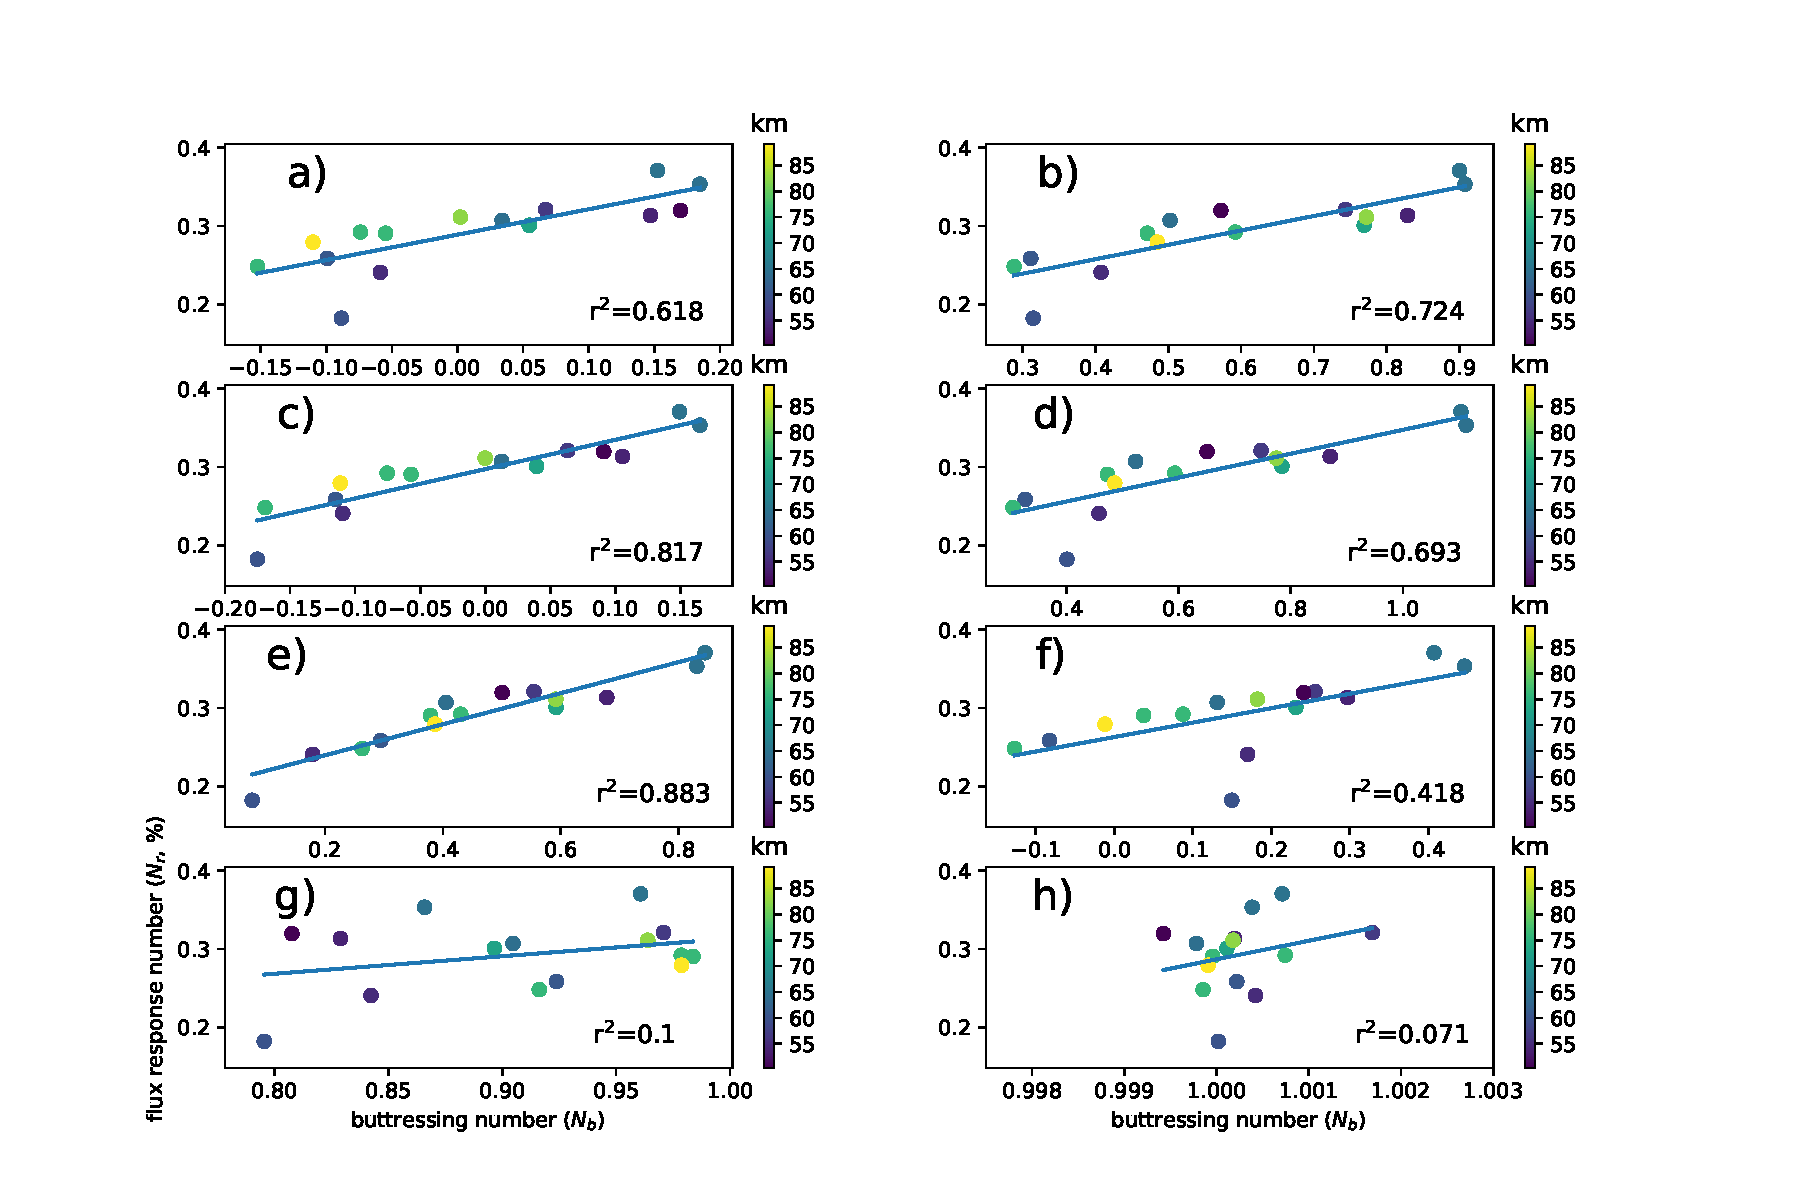
\includegraphics[width=1\linewidth]{figs/diffStressCompAvgL.pdf}
\caption{The relationships between grounding line flux response number ($N_r$) and eight different stress components, $\sigma_f$ (a), $\sigma_{af}$ (b), $\sigma_{p1}$ (c), $\sigma_{p2}$ (d), $\sigma_{x}$ (e), $\sigma_{y}$ (f), $\sigma_{s}$ (g) and $\sigma_h$ (h). See Table \ref{stressDef} for the definition of each stress component in the Larsen C 20 km $\times$ 20 km box experiments. The color bars show the values of $dG$ for each perturbation spot.}
\label{diffStressCompAvgL}
\end{figure}

%Figure \ref{fig1} shows the relationships of integrated GL flux change and various buttressing numbers for different stresses for all perturbations over the MISMIP+ ice shelf. The inherent pattern is ambiguous. However, if we look closely to the distances of the perturbation points to GL, we can see the far scattered points are mostly near to the GL. Figure \ref{fig2} is an example of the impact of perturbation location on the velocity changes across the ice shelf and on GL. In addition to the complex velocity change patterns around the perturbation location, there are two clear patterns we can find: 1) the magnitude of vel. change decreased with distances away from the perturbation and 2) the vel. change pattern is different when the perturbation approaches to the GL. 

%The first one is easy to understand as the energy of perturbation decreases when it propagate away to far upstream and downstream. The second one can be explained by at least two mechanisms: 1) ice dynamics are more remarkably impacted by the grounded ice flow near the GL and 2) the propagation of perturbation can be more impacted by the spatial GL geometry. These two impacts can be confirmed if we remove the perturbation points both near the GL and in the open ice shelf area (little buttressing). See Figure \ref{fig3}, we only keep the perturbation points that are > 5 km away from the GL and also their x coordinates are < km 480 and some clear trends starts to appear. The buttressing number for shear and hoop stress seems to be not good metrics, but there are some relationships for $\sigma_{p1}$, $\sigma_{p2}$, $\sigma_f$, $\sigma_{af}$, $\sigma_x$ and $\sigma_y$, especially for $\sigma_{p1}$. 

%This can be further verified if we apply the perturbation to a spatial box (20km by 20 km) and calculate the average stress field in each perturbation box, by which we can smooth out and decrease the impacts of distances on the GL flux responses (Fig \ref{fig4}). the shear stress buttressing number is still a bad metric, but the averaged hoop stress turns out to become much better than the 2 km perturbation cell case. Other stresses along different directions also present better behaviors for GL flux responses.

%Based on the above MISMIP+ results, we apply the same approaches to Larsen C ice shelf. See Figure \ref{fig5}, though Larsen C has a more complex geometry compared to MISMIP+, it still show good linear relationship between the $\sigma_{p1}$ buttressing number and GL flux response. Different than the MISMIP+ runs, we remove the perturbation spots that are < 10km to the GL and calving front.



\section{Discussions}

Based on the above discussion we hypothesize that the two main factors controlling how a local perturbation in ice shelf thickness leads to changes in ice flux across the GL are 1) the distance between a perturbation location and the GL and 2) the first principle stress at the perturbation location. Figure \ref{distPerturbComp} shows an example of the impact of the perturbation location on the velocity changes across the ice shelf and GL. Despite the complex patterns of velocity change around the perturbation spot, we can see two clear features: 1) the magnitude of velocity change decreases with distances away from the perturbation spot and 2) the velocity change pattern becomes different and more disordering when the perturbation  approaches to GL. 

\begin{figure}
	\centering
	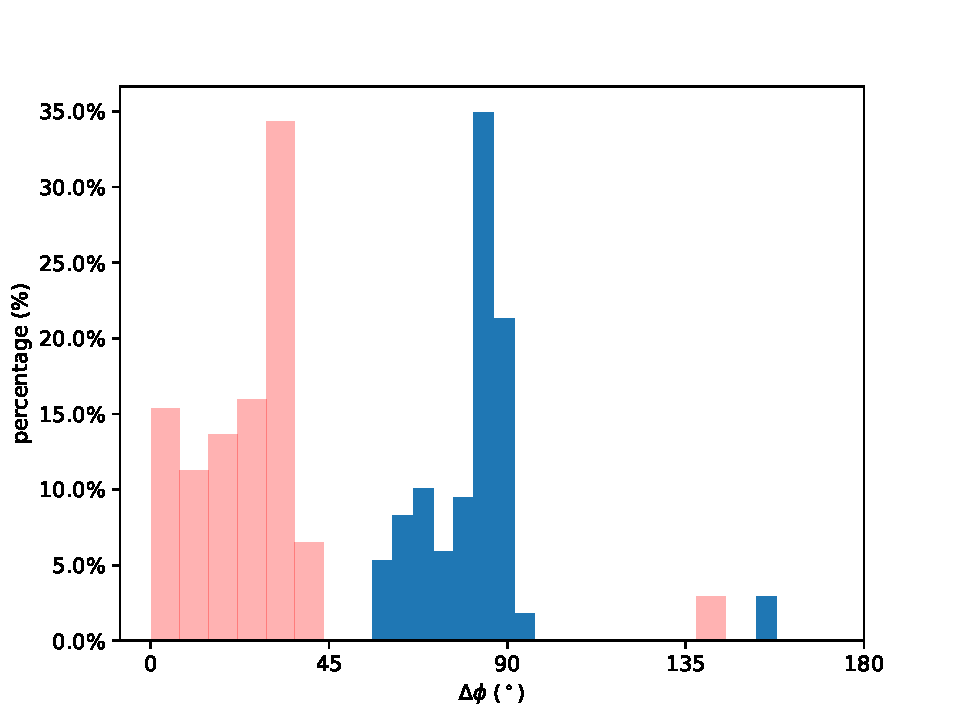
\includegraphics[width=1\linewidth]{figs/perturb_theta_velchange.pdf}
	\caption{An example of ice speed changes (\%) across the MISMIP+ ice shelf and grounding line after apply the perturbations at different locations (blue circles).}
	\label{distPerturbComp}
\end{figure}

The first feature is easy to understand because the energy of perturbation decays as it propagate away to far upstream and downstream. However, the perturbation propagation is not simply dependent on distance, but replies on the ice flow field. A complete perturbation propagation theory is necessary to describe/explain these small velocity changes across the ice shelf, however, it is beyond the scope of this study. The second one can probably be explained by two ice-flow mechanisms: 1) ice shelf dynamics are remarkably impacted by the grounded ice flow near the GL since it's a coupled system for grounded ice sheet and floating ice shelf and in MALI they is resolved as an integrated system as well; 2) the propagation of perturbation can be impacted by the spatial GL geometry. For example, the perturbation in Figure \ref{distPerturbComp}a can not directly impact the ice on the other side of the grounded peninsula in the same way as for it's neighboring cells.

In addition, the impacts of distance can also be verified from the box averaging experiments (Figure \ref{diffStressCompAvg} and \ref{diffStressCompAvgL}). By smoothing out the stresses in the perturbation box, different distances to GL for each cells and their impacts in the perturbation box are also averaged, resulting in better linear $N_b$-$N_r$ relationships. This possibly indicates that those linear $N_b$-$N_r$ relationships can apply for realistic ice shelves, as in reality the basal melting always occurs in wide spatial regions.

%These two impacts can be confirmed if we remove the perturbation points both near the GL and in the open ice shelf area (little buttressing). See Figure \ref{fig3}, we only keep the perturbation points that are > 5 km away from the GL and also their x coordinates are < km 480 and some clear trends starts to appear. The buttressing number for shear and hoop stress seems to be not good metrics, but there are some relationships for $\sigma_{p1}$, $\sigma_{p2}$, $\sigma_f$, $\sigma_{af}$, $\sigma_x$ and $\sigma_y$, especially for $\sigma_{p1}$. 

It is still not very clear why the integrated GL flux change is strongly correlated to the first principle stress at the perturbation location than other stress components (especially the second principle stress). We can find some clues by looking at the difference of $\sigma_{p1}$, $\sigma_{p2}$, $\sigma_f$ and $\sigma_s$ along GL before and after applying the perturbation (Fig \ref{stressDiff}). Clearly, the distribution of the difference of $\sigma_{p1}$ across ice shelf is less disordering than that of $\sigma_{p2}$, $\sigma_{f}$ and $\sigma_{s}$. This indicates that the propagation of the perturbation for different stress components can be greatly varied in patial, which is probably the main reason of those different $N_b$-$N_r$ relationships for different stress components. A further evidence of this explanation can be found in Figure \ref{stressDiff_velDiff}, where we show the changes of veocity and stress components on GL. Clearly, the change of ice speeds at GL is more relevant to of $\sigma_{p1}$ and $\sigma_{f}$, compared to $\sigma_{p2}$ and $\sigma_{s}$. This possibly indicate that the changes of ice velocity under small basal perturbations may be more likely controlled by the changes of the stress components that are more aligned with ice flow directions.


Therefore, we can find similar patterns for shear stress $\sigma_s$. The ice flow for most parts of MISMIP+ and Larsen C ice shelf are divergent, which in practical don't supply any buttressing to resist along flow. Since the hoop stress is quite small (Fig \ref{diffStressCompAvg}h and Fig \ref{diffStressCompAvgL}h), the main source of buttressing arises from the shear flow of ice shelf (assume the buttressing is proportional to the magnitude of $\sigma_{obj}$). This can be confirmed in \citep{furst2016} where we can clearly see that some non-passive (with buttressing) ice shelf are purely extensive regime. Similar to the case of $\sigma_{p2}$, the complex spatial propagation of the perturbed stress change from the perturbation spot to GL is a possible cause.



\begin{figure}
	\centering
	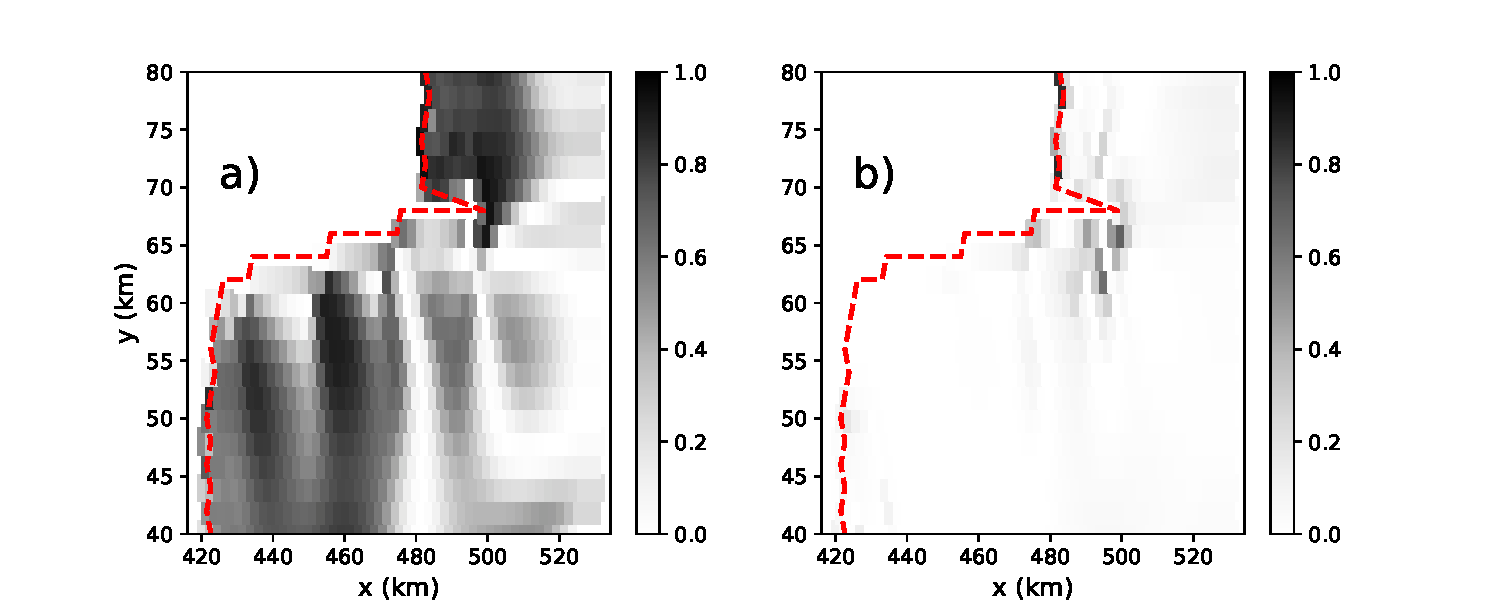
\includegraphics[width=1\linewidth]{figs/stressDiff_velDiff_GL_allPerturb.pdf}
	\caption{The change percentage of ice speed (blue dots) and stress components (red dots; a--d represents $\sigma_{p1}$, $\sigma_{p2}$, $\sigma_{f}$ and $\sigma_{s}$, respectively) for all cells at the grounding line corresponding to Figure \ref{stressDiff}.}
	\label{stressDiff_velDiff}
\end{figure}

%From Figure \ref{fig2} we can see the ice vel. change over ice shelf and GL depends on the relative location to GL position. When p is near the center of the ice shelf, the ice flux change is more predictable than p close to the GL. The magnitude of vel. change decrease with distance, and the vel. upstream (downstream) tends to show an increase (decrease). For the ice shelf (GL) upstream to the perturbation, a decrease of ice thickness indicates a decrease of buttressing, however, for ice shelf downstream to the perturbation, it means a decrease of driving stress. This pattern become ambiguous when the perturbation is close to GL as it's dynamics is more affected by the grounded ice sheet. 


Though there is no clear linear $N_b$-$N_r$ relationships near GL, the integrated GL flux mainly depends on the GL flux of cells that are close to the perturbation spot. From Figure \ref{stndVarFluxP}b, we can see that for perturbations near GL, their impacts are mainly local and thus can only affect their neighboring ice streams, which can possibly enhance the spatial heterogeneity of marine ice sheet responses under ocean warming forcings.  


\section{Conclusions}

From this study we find that the sensitivity of grounding line (GL) flux to melt perturbations beneath ice shelves appears to be linearly related to the buttressing number for certain stress field of the ice flow regime when the perturbations are located near the center of ice shelves. We can divide an ice shelf into three different geometric regions: 1) near GL where the shear margins dominate; 2) near the calving fronts where ice can be considered as ``passive'' and 3) the central regions of ice shelf. Though it is ambiguous to indentify the boundaries of those three sub-regions, we find that both the shear margins and passive ice regions show very weak linear connections to GL flux changes. The shear margins are strongly impacted by the upstream grounded stream flows and the passive ice shelf basically has negligible contribution to GL dynamics. 

The buttressing of ice shelf resists ice flows from upstream. The maximum buttressing number (calculated from the second principle stress $\sigma_{p2}$) is a commonly used metric to quantify the buttressing effects of ice shelf, doesn't show clear correlations to the changes of GL flux. Among many possible factors we find that the distance away from perturbation locations may be a critical control for perturbation propagation across ice shelves, which is important for understanding the relationships between the stress field of the ice shelf and the GL flux changes. The GL ice speed changes may be more correlated to the changes of the first principle stress ($\sigma_{p1}$) and normal stress along flow ($\sigma_{f}$) than other stress components, for example, the second principle stress ($\sigma_{p2}$) and the shear stress ($\sigma_s$), indicating that the stress component ($\sigma_{p2}$) that contribute significantly to buttressing is not necessarily related to the progapation of buttressing. 

The linear $N_b$-$N_r$ relationships presented in this study are based on small (1 m) thickness perturbations. However, it's still unclear if they can stand for large melts at the bottom of ice shelves ({\bf{Perhaps we also need to do large perturbation experiments?}}). Despite the progress we have made in this study, we suggest to apply a fully-developed perturbation propagation model for further understanding the physics of GL flux changes under ocean forcings. 

\section{Acknowledgement}
\bibliographystyle{igs}
\bibliography{refs}

\section{Appendix}

%\renewcommand\thefigure{\thesection.\arabic{figure}}  
\renewcommand{\thefigure}{A\arabic{figure}}
\setcounter{figure}{0}

\begin{figure}
	\centering
	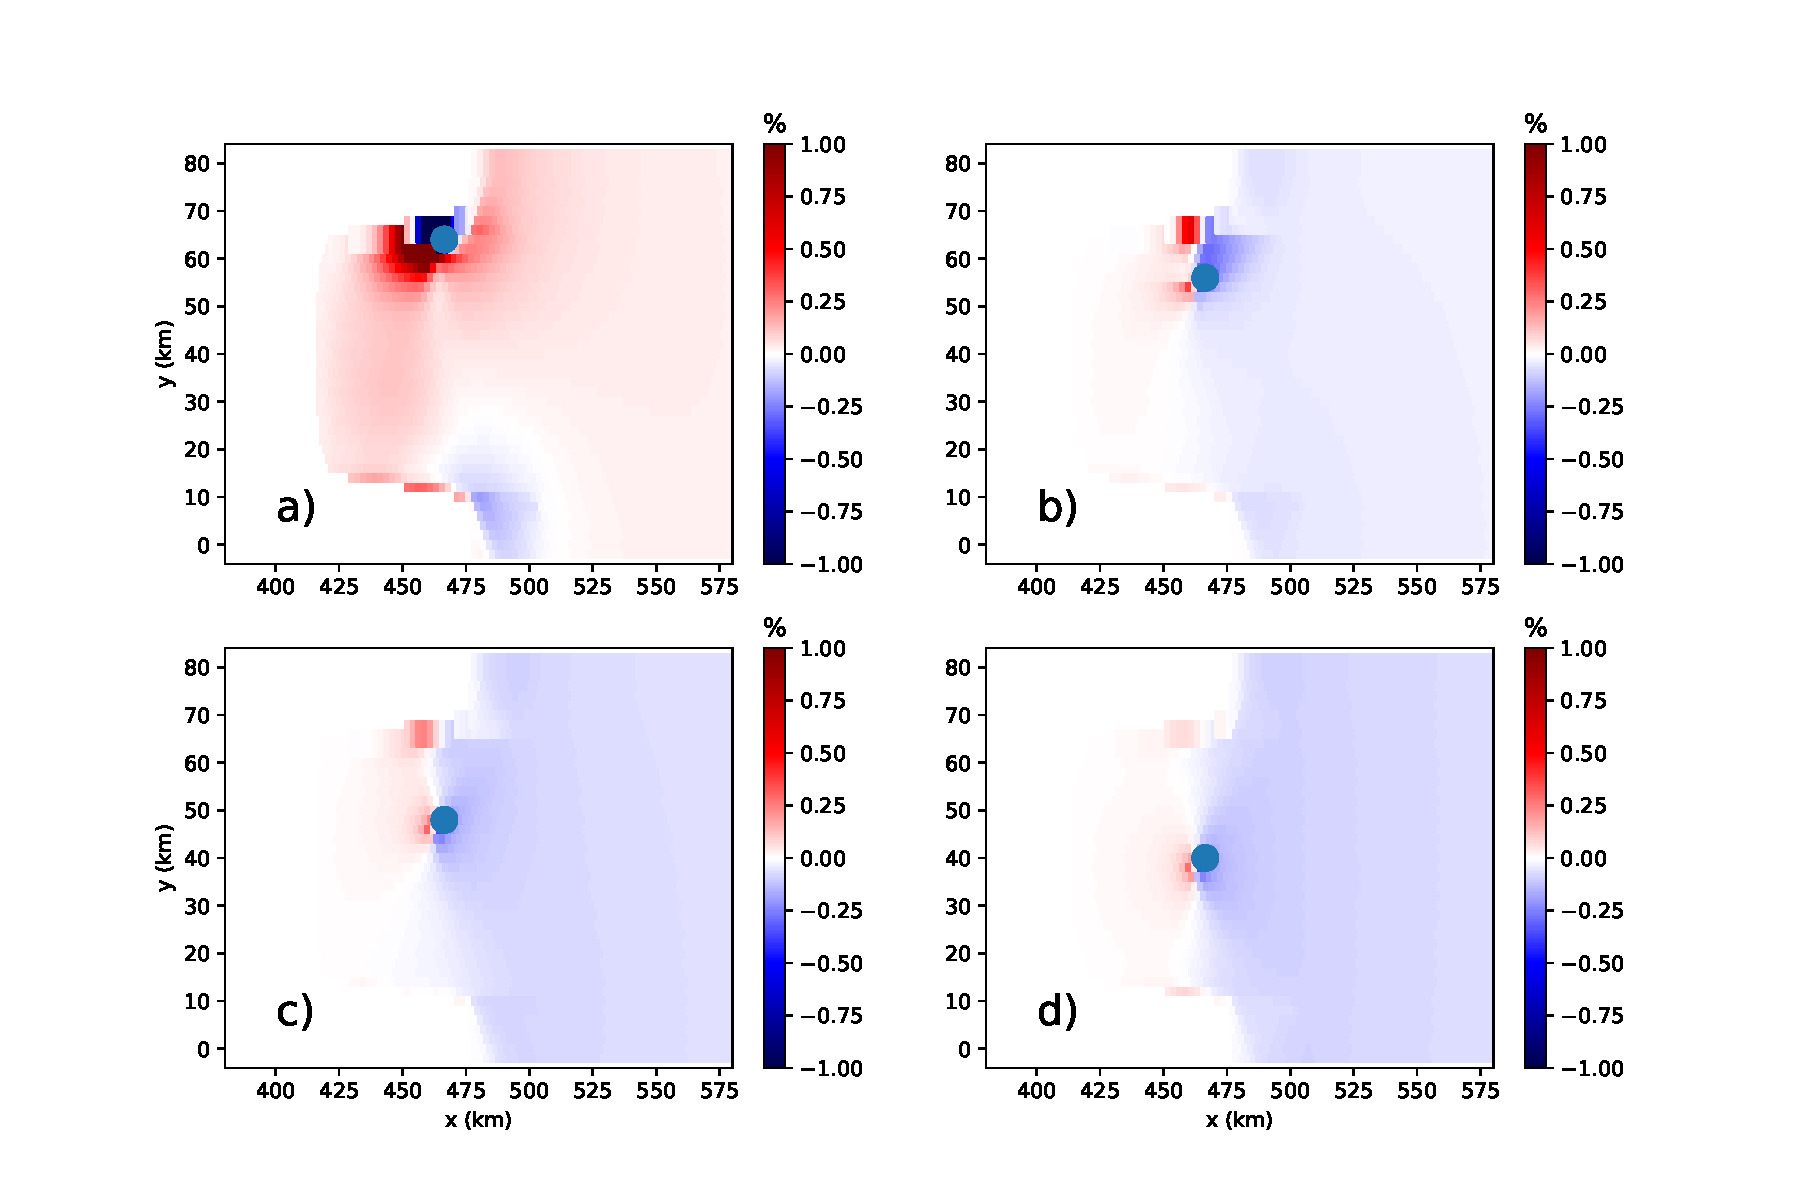
\includegraphics[width=1\linewidth]{figs/distPerturbComp.pdf}
	\caption{An example of ice speed changes (\%) across the MISMIP+ ice shelf and grounding line after apply the perturbations at different locations (blue circles).}
	\label{distPerturbComp}
\end{figure}

\begin{figure}
	\centering
	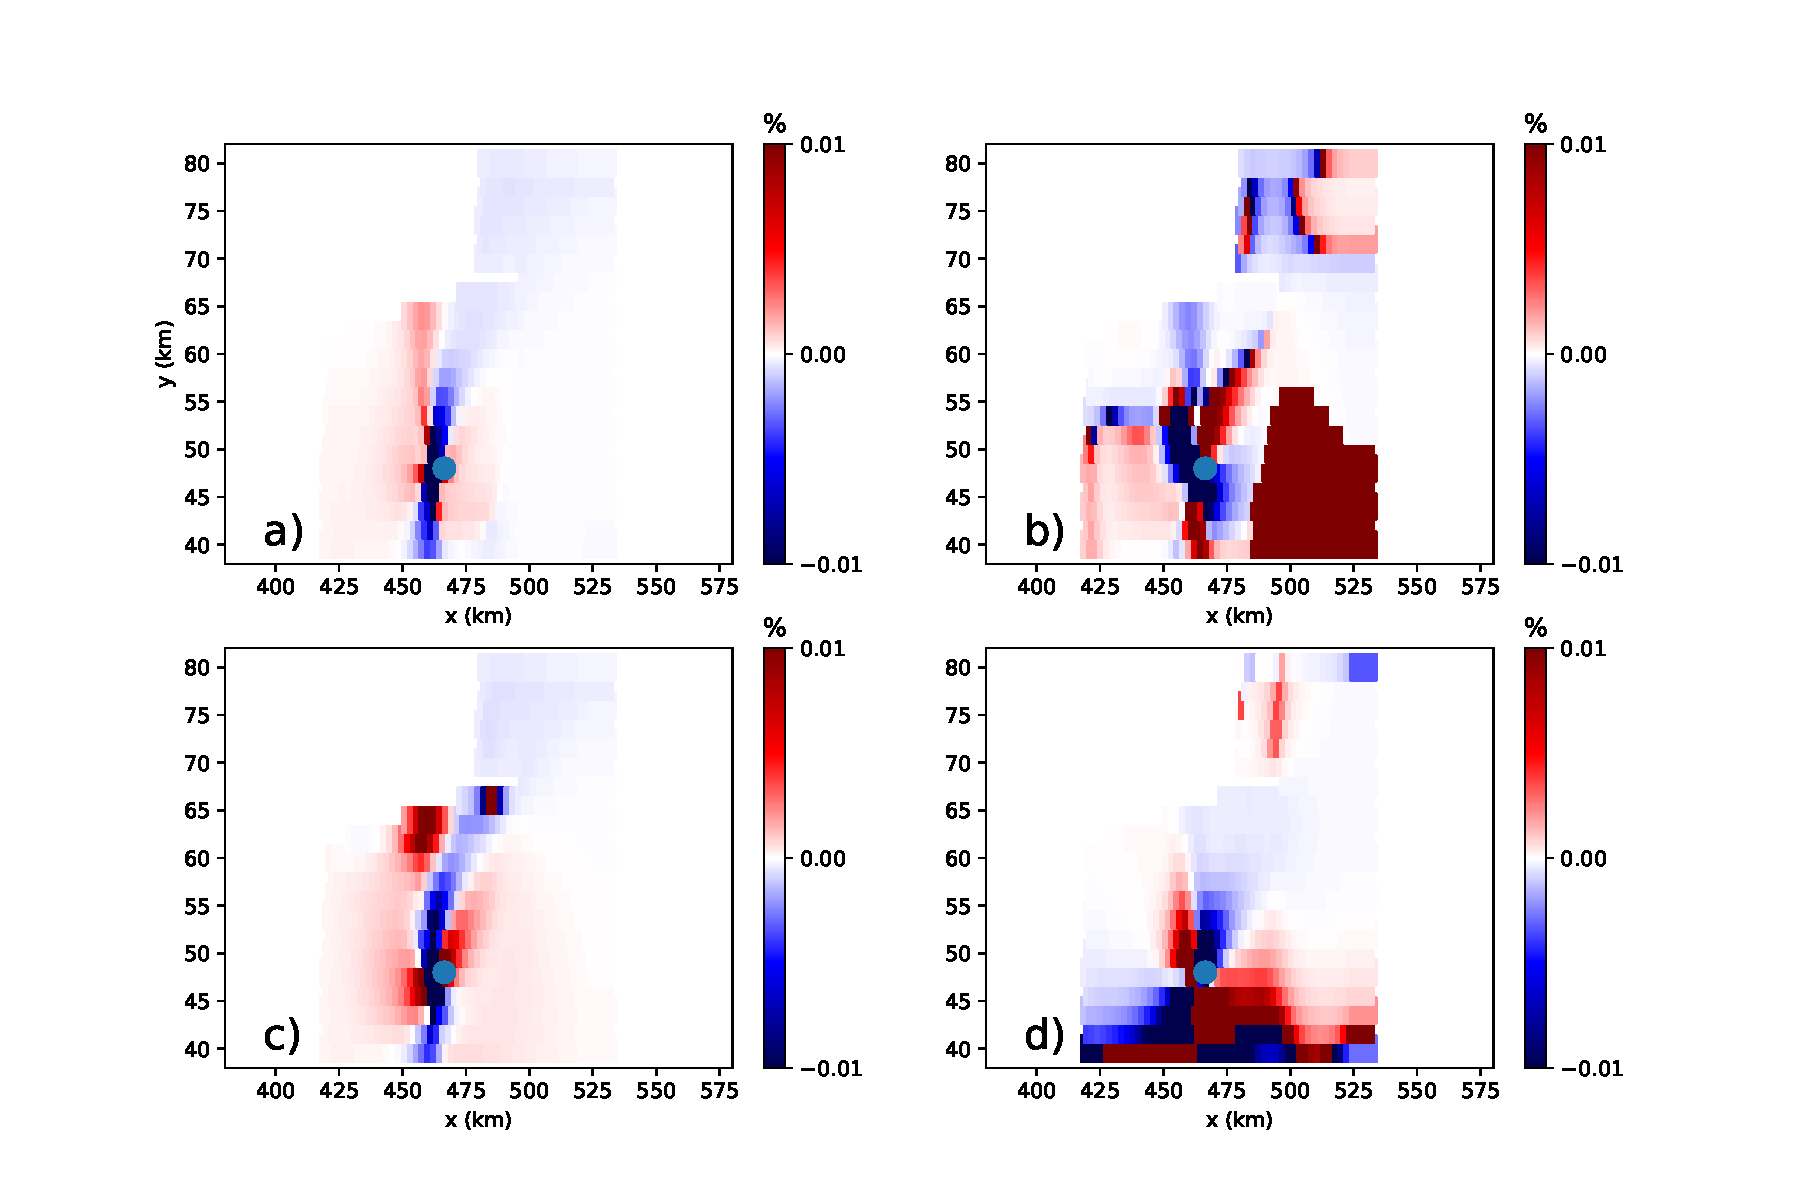
\includegraphics[width=1\linewidth]{figs/stressDiff.pdf}
	\caption{An example of stress component changes (\%) across the MISMIP+ ice shelf and grounding line after apply the perturbations at different locations (blue circles). (a) Changes of $\sigma_{p1}$; (b) Changes of $\sigma_{p2}$; (c) Changes of $\sigma_{f}$; (d) Changes of $\sigma_{s}$;.}
	\label{stressDiff}
\end{figure}

\begin{figure}
	\centering
	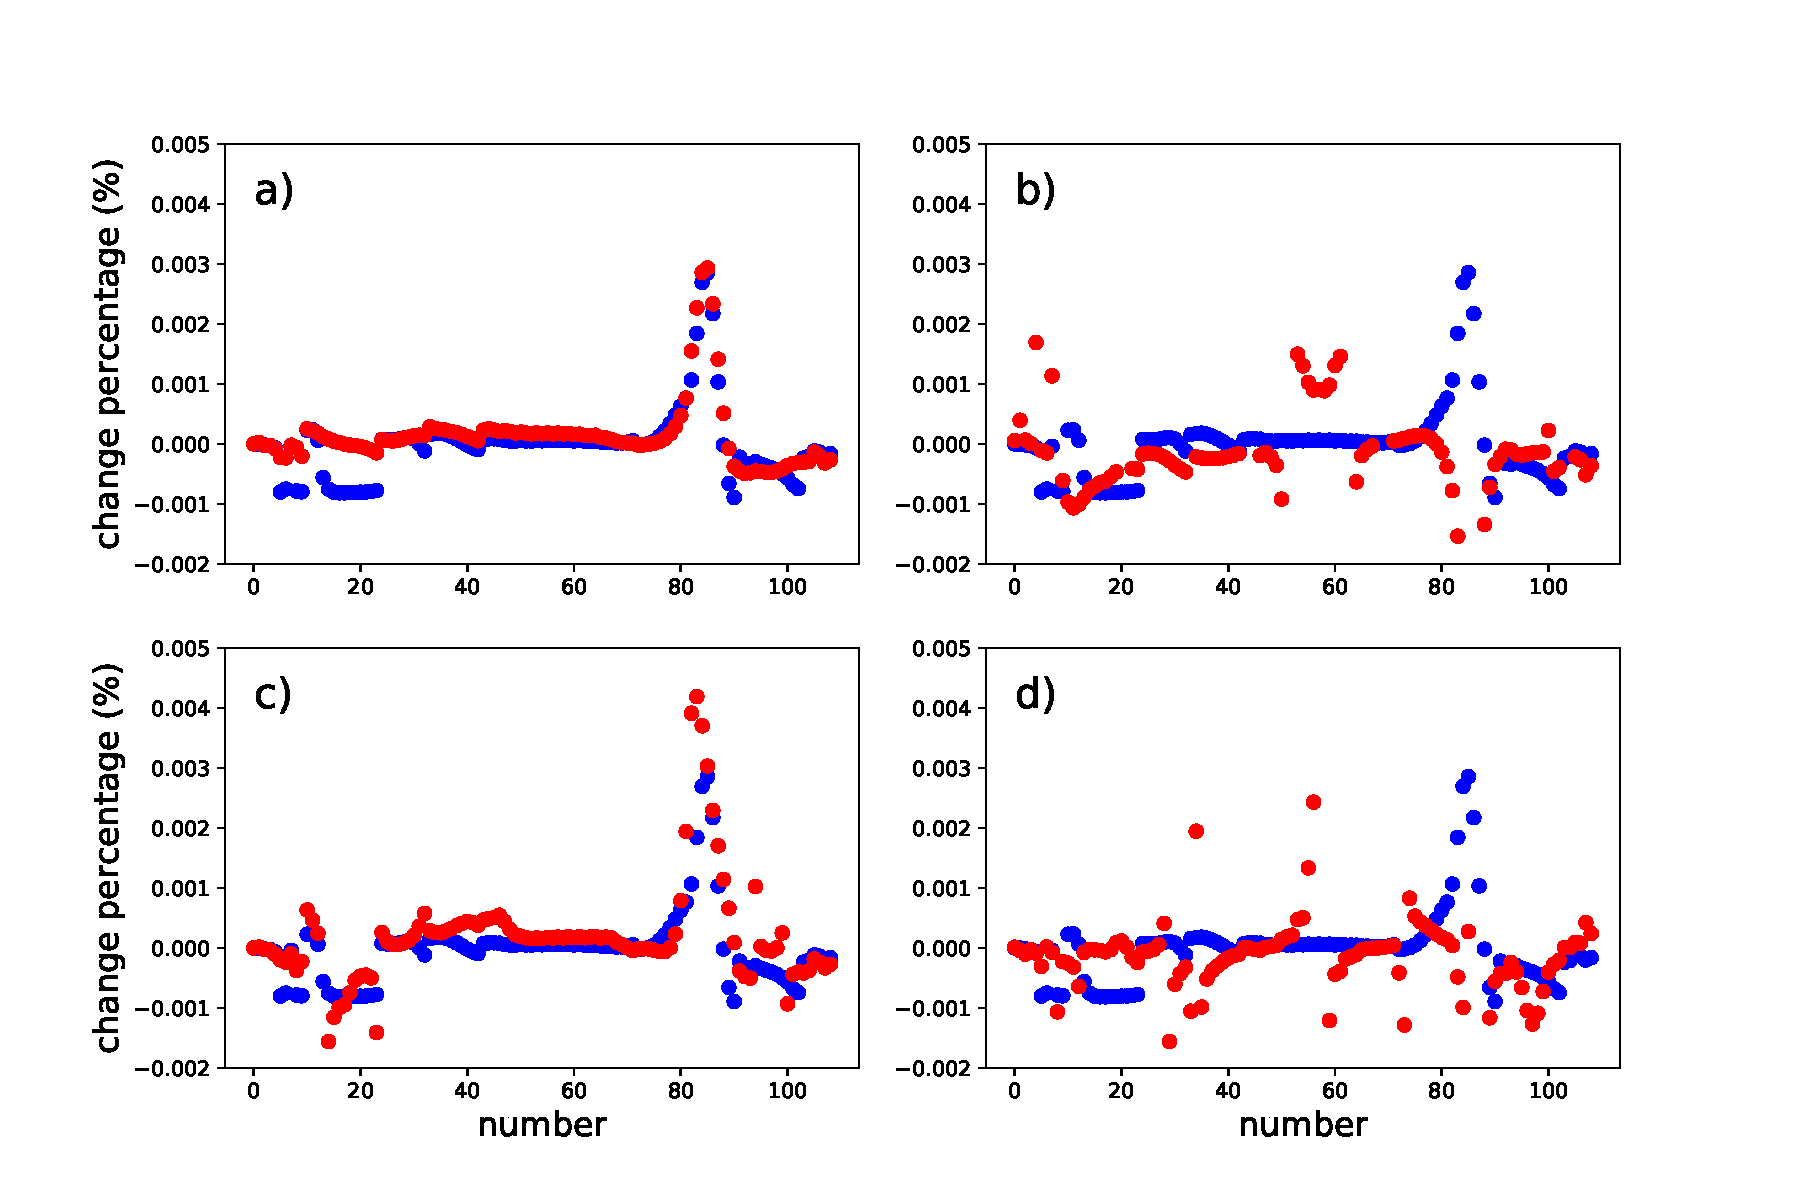
\includegraphics[width=1\linewidth]{figs/diffStress_diffVel.pdf}
	\caption{The change percentage of ice speed (blue dots) and stress components (red dots; a--d represents $\sigma_{p1}$, $\sigma_{p2}$, $\sigma_{f}$ and $\sigma_{s}$, respectively) for all cells at the grounding line corresponding to Figure \ref{stressDiff}.}
	\label{stressDiff_velDiff}
\end{figure}

\end{document}
